% SOURCE_AUTHORITY: sga5_fr_workpass.tex, lines 2894--3282 (LF-normalized unit).
% SOURCE_SHA256: 791F4EFFC5E02832D5D77ED03518C8156D6F07E4C8238B03545DB93D883FBB28
\begin{statement}{Teorema 4.4}
Sejam, para $i=1,2$, $f_i:X_i\longrightarrow Y_i$ um $S$-morfismo próprio,
\[
f=f_1\times_S f_2:X\longrightarrow Y,\qquad
p_i:X\longrightarrow X_i,\qquad q_i:Y\longrightarrow Y_i
\]
as projeções. Seja, por outro lado,
\begin{equation}
\tag{4.4.0}
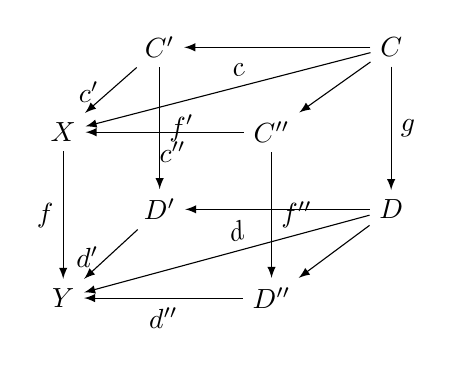
\begin{tikzpicture}[>=latex,baseline=(current bounding box.center),scale=0.98]
\node (Cp) at (0,2.1) {$C'$};
\node (C) at (3.0,2.1) {$C$};
\node (X) at (-1.25,1.0) {$X$};
\node (Cpp) at (1.45,1.0) {$C''$};
\node (Dp) at (0,0) {$D'$};
\node (D) at (3.0,0) {$D$};
\node (Y) at (-1.25,-1.15) {$Y$};
\node (Dpp) at (1.45,-1.15) {$D''$};
\draw[->] (C) -- (Cp);
\draw[->] (Cp) -- node[left,pos=.55] {$c'$} (X);
\draw[->] (C) -- node[above,sloped,pos=.45] {$c$} (X);
\draw[->] (C) -- (Cpp);
\draw[->] (Cpp) -- node[below,pos=.45] {$c''$} (X);
\draw[->] (Cp) -- node[right] {$f'$} (Dp);
\draw[->] (Cpp) -- node[right] {$f''$} (Dpp);
\draw[->] (C) -- node[right] {$g$} (D);
\draw[->] (X) -- node[left] {$f$} (Y);
\draw[->] (D) -- (Dp);
\draw[->] (Dp) -- node[left,pos=.55] {$d'$} (Y);
\draw[->] (D) -- node[above,sloped,pos=.45] {$d$} (Y);
\draw[->] (D) -- (Dpp);
\draw[->] (Dpp) -- node[below] {$d''$} (Y);
\end{tikzpicture}
\end{equation}
um cubo comutativo cujas faces horizontais são cartesianas, com $c'$, $c''$, $d'$, $d''$ próprios. Ponhamos
\[
c_i'=p_i c',\qquad c_i''=p_i c'',\qquad d_i'=q_i d',\qquad d_i''=q_i d''.
\]
Por fim, sejam $L_i\in\ob \Dctf(X_i)$. Tem-se então um quadrado comutativo
\begin{equation}
\tag{4.4.1}
\begin{tikzcd}[column sep=huge,row sep=huge]
f_*c'_*\uRHom(c_1'{}^*L_1,c_2'{}^!L_2)\otimes^{\mathbf L}
f_*c''_*\uRHom(c_2''{}^*L_2,c_1''{}^!L_1)
 \arrow[r,"(1)"] \arrow[d,"(2)"'] &
f_*c_*K_C \arrow[d,"(4)"] \\
d'_*\uRHom(d_1'{}^*M_1,d_2'{}^!M_2)\otimes^{\mathbf L}
d''_*\uRHom(d_2''{}^*M_2,d_1''{}^!M_1)
 \arrow[r,"(3)"'] &
d_*K_D ,
\end{tikzcd}
\end{equation}
onde $M_i=f_{i*}L_i$, $(3)$ é dada por 4.2.4, $(1)$ deduz-se de 4.2.4 aplicando $f_*$ e compondo com a flecha canônica
\[
f_*c'_*(-)\otimes^{\mathbf L} f_*c''_*(-)\longrightarrow f_*(c'_*(-)\otimes^{\mathbf L}c''_*(-)),
\]
$(2)$ é o produto tensorial das flechas 3.7.5 relativas às faces que contêm $f$, e $(4)$ é definida pela flecha de adjunção $g_*K_C=g_!g^!K_D\longrightarrow K_D$.
\end{statement}

\begin{prooftext}[Demonstração]
Ponhamos
\[
DL_1\otimes_S^{\mathbf L}L_2=P,\qquad
L_1\otimes_S^{\mathbf L}DL_2=Q,\qquad
DM_1\otimes_S^{\mathbf L}M_2=E,\qquad
M_1\otimes_S^{\mathbf L}DM_2=F.
\]
Consideremos o diagrama
\begin{equation}
\tag{4.4.2}
\begin{tikzcd}[column sep=2.6em,row sep=2.6em,cells={nodes={font=\scriptsize}}]
f_*c'_*c'{}^!P\otimes^{\mathbf L} f_*c''_*c''{}^!Q
  \arrow[rr,"(1)"] \arrow[d,"(8)"'] &&
f_*c_*c^!\bigl(P\otimes^{\mathbf L}Q\bigr)
  \arrow[r,"(2)"] \arrow[d,"(9)"'] &
f_*c_*c^!K_X \arrow[d,"(10)"]\\
d'_*d'{}^!f_*P\otimes^{\mathbf L}d''_*d''{}^!f_*Q
  \arrow[r,"(3)"'] \arrow[d,"(11)"'] &
d_*d^!\bigl(f_*P\otimes^{\mathbf L}f_*Q\bigr)
  \arrow[r,"(4)"'] \arrow[d,"(12)"'] &
d_*d^!f_*\bigl(P\otimes^{\mathbf L}Q\bigr)
  \arrow[r,"(5)"'] &
d_*d^!f_*K_X \arrow[d,"(13)"]\\
d'_*d'{}^!E\otimes^{\mathbf L}d''_*d''{}^!F
  \arrow[r,"(6)"'] &
d_*d^!\bigl(E\otimes^{\mathbf L}F\bigr)
  \arrow[rr,"(7)"'] &&
d_*d^!K_Y,
\arrow[from=1-1,to=2-2, phantom, "\scriptstyle (A)"]
\arrow[from=1-3,to=2-4, phantom, "\scriptstyle (B)"]
\arrow[from=2-1,to=3-2, phantom, "\scriptstyle (C)"]
\arrow[from=2-2,to=3-4, phantom, "\scriptstyle (D)"]
\end{tikzcd}
\end{equation}
onde as flechas são as seguintes: $(1)$ deduz-se de 4.2.2 aplicando $f_*$, $(2)$ é definida por 4.1.2, $(3)$ é dada por 4.2.2, $(4)$ pela flecha canônica $f_*P\otimes^{\mathbf L}f_*Q\longrightarrow f_*(P\otimes^{\mathbf L}Q)$, $(5)$ por 4.1.2, $(6)$ por 4.2.2, $(7)$ por 4.1.2, $(8)$ é o produto tensorial das flechas 3.7.3, $(9)$ e $(10)$ são definidas por 3.7.3, $(11)$ e $(12)$ pelos isomorfismos $f_*P\longrightarrow E$, $f_*Q\longrightarrow F$ (3.3.1), e $(13)$ pela flecha de adjunção $f_*K_X\longrightarrow K_Y$. Por definição, 4.4.1 identifica-se, por 3.1.1 e 3.2.1, com a borda exterior de 4.4.2. Basta, portanto, provar que os quadrados $(A)$, $(B)$, $(C)$, $(D)$ são comutativos. A comutatividade de $(B)$ e $(C)$ é evidente pela funtorialidade. Resta demonstrar a de $(A)$ e $(D)$.

a) Comutatividade de $(D)$. Basta provar que o quadrado
\begin{equation}
\tag{4.4.3}
\begin{tikzcd}[column sep=large,row sep=large]
f_*P\otimes^{\mathbf L}f_*Q \arrow[r] \arrow[d] & f_*K_X \arrow[d]\\
E\otimes^{\mathbf L}F \arrow[r] & K_Y
\end{tikzcd}
\end{equation}
(correspondente a $(D)$ para $d=\Id$) é comutativo. Recordemos que o emparelhamento
\[
P\otimes^{\mathbf L}Q\longrightarrow K_X
\quad(\text{resp. }E\otimes^{\mathbf L}F\longrightarrow K_Y)
\]
é o produto tensorial externo das flechas de avaliação
\[
DL_i\otimes^{\mathbf L}L_i\longrightarrow K_{X_i}
\quad(\text{resp. }DM_i\otimes^{\mathbf L}M_i\longrightarrow K_{Y_i}).
\]
Pelos isomorfismos de Künneth
\[
f_{1*}DL_1\otimes_S^{\mathbf L} f_{2*}L_2 \lisom f_*P,\qquad
f_{1*}L_1\otimes_S^{\mathbf L} f_{2*}DL_2 \lisom f_*Q,
\]
4.4.3 identifica-se, portanto, com o produto tensorial externo dos quadrados
\begin{equation}
\tag{4.4.4}
\begin{tikzcd}[column sep=large,row sep=large]
f_{i*}DL_i\otimes^{\mathbf L} f_{i*}L_i
 \arrow[r,"(1)"] \arrow[d,"(3)"'] &
f_{i*}K_{X_i} \arrow[d,"(4)"]\\
DM_i\otimes^{\mathbf L}M_i \arrow[r,"(2)"'] & K_{Y_i},
\end{tikzcd}
\end{equation}
onde $(2)$ é a flecha de avaliação, $(1)$ a composição da flecha canônica
\[
f_{i*}DL_i\otimes^{\mathbf L} f_{i*}L_i\longrightarrow f_{i*}(DL_i\otimes^{\mathbf L}L_i)
\]
e da flecha definida pela flecha de avaliação, $(3)$ é o produto tensorial do isomorfismo de dualidade $f_{i*}DL_i\longrightarrow DM_i$ e da flecha identidade de $M_i$, e $(4)$ é a flecha de adjunção. Basta, portanto, verificar a comutatividade dos quadrados 4.4.4. Como o isomorfismo de dualidade anterior é a composição da flecha canônica (SGA 4 XVIII 3.1.9.5)
\[
f_{i*}\uRHom(L_i,K_{X_i})\longrightarrow \uRHom(f_{i*}L_i,f_{i*}K_{X_i})
\]
e da flecha deduzida da flecha de adjunção
\[
f_{i*}K_{X_i}\longrightarrow K_{Y_i},
\]
basta ver que o seguinte quadrado é comutativo:
\begin{equation}
\tag{4.4.5}
\begin{tikzcd}[column sep=large,row sep=large]
f_{i*}\uRHom(L_i,K_{X_i})\otimes^{\mathbf L} f_{i*}L_i
 \arrow[r,"(1)"] \arrow[d,"(3)"'] &
f_{i*}K_{X_i} \arrow[d,"\Id"]\\
\uRHom(f_{i*}L_i,f_{i*}K_{X_i})\otimes^{\mathbf L} f_{i*}L_i
 \arrow[r,"(2)"'] &
f_{i*}K_{X_i},
\end{tikzcd}
\end{equation}
onde $(1)$ é a flecha $(1)$ de 4.4.4, $(2)$ é a flecha de avaliação, e $(3)$ é o produto tensorial por $f_{i*}L_i$ da flecha canônica que acabamos de mencionar. Mais geralmente, para toda flecha $N_i\longrightarrow f_{i*}L_i$ de $\Dctf(X_i)$, isto é, toda flecha $L_i\xrightarrow{u}N_i$ de tipo $1$ sobre $f_i$, o triângulo
\[
\begin{tikzcd}[column sep=large,row sep=large]
f_{i*}\uRHom(L_i,K_{X_i})\otimes^{\mathbf L}N_i
 \arrow[dr] \arrow[d] & \\
\uRHom(N_i,f_{i*}K_{X_i})\otimes^{\mathbf L}N_i \arrow[r] &
f_{i*}K_{X_i}
\end{tikzcd}
\]
deduzido de 4.4.5 é comutativo: de fato, por funtorialidade, pode-se supor que $L_i=f_i^*N_i$, com $u$ dado pela identidade de $L_i$; a flecha
\[
f_{i*}\uRHom(L_i,K_{X_i})\longrightarrow\uRHom(N_i,f_{i*}K_{X_i})
\]
é então a inversa do isomorfismo de dualidade trivial, e a comutatividade do triângulo verifica-se imediatamente no nível dos complexos, tomando uma resolução plana de $N_i$ e uma resolução injetiva de $K_{X_i}$.

b) Comutatividade de $(A)$. Remetendo-nos à definição de 3.7.3, vemos que basta verificar essa comutatividade em cada um dos seguintes casos:
\[
\text{(i) } X_i=Y_i,\quad f_i=\text{flecha identidade de }X_i;\qquad
\text{(ii) as faces laterais de 4.4.0 são cartesianas.}
\]
Situemo-nos no caso (i). O quadrado $(A)$ é a borda exterior do diagrama
\[
\begin{tikzcd}[column sep=large,row sep=large]
c'_*c'{}^!P\otimes^{\mathbf L}c''_*c''{}^!Q
 \arrow[r,"\sim"] \arrow[d,"(8)"'] &
c_*\bigl(c'{}^!P\otimes_X^{\mathbf L}c''{}^!Q\bigr)
 \arrow[r] \arrow[d] &
c_*c^!(P\otimes^{\mathbf L} Q)\arrow[d,"(9)"]\\
d'_*d'{}^!P\otimes^{\mathbf L}d''_*d''{}^!Q
 \arrow[r,"\sim"'] &
d_*\bigl(d'{}^!P\otimes_X^{\mathbf L}d''{}^!Q\bigr)
 \arrow[r] &
d_*d^!(P\otimes Q),
\arrow[from=1-1,to=2-2, phantom, "\scriptstyle A_1"]
\arrow[from=1-2,to=2-3, phantom, "\scriptstyle A_2"]
\end{tikzcd}
\]
no qual os isomorfismos horizontais de $A_1$ são isomorfismos de Künneth, as flechas horizontais de $A_2$ são dadas por 4.2.1, e a flecha vertical central deduz-se aplicando $d_*$ à flecha
\[
g_!(c'{}^!P\otimes_X^{\mathbf L}c''{}^!Q)\longrightarrow d'{}^!P\otimes_X^{\mathbf L}d''{}^!Q
\]
definida, por Künneth, pelo produto tensorial externo das flechas de adjunção
\[
f'_!c'{}^!P\longrightarrow d'{}^!P,\qquad
f''_!c''{}^!Q\longrightarrow d''{}^!Q.
\]
Ora, essas flechas de adjunção e as flechas identidade de $d'_!d'{}^!P$, $d''_!d''{}^!Q$ definem triângulos comutativos de flechas de tipo $3$ (1.4)
\[
\begin{tikzcd}[column sep=large,row sep=large]
& c'{}^!P \arrow[d] \arrow[dl] & & c''{}^!Q \arrow[d]\arrow[dl]\\
d'_!d'{}^!P & d'{}^!P\arrow[l] & d''_!d''{}^!Q & d''{}^!Q\arrow[l]
\end{tikzcd}
\]
sobre
\[
\begin{tikzcd}[column sep=large,row sep=large]
& C' \arrow[d,"f'"] \arrow[dl,"c'"']\\
X & D'\arrow[l,"d'"]
\end{tikzcd}
\qquad
\begin{tikzcd}[column sep=large,row sep=large]
& C'' \arrow[d,"f''"] \arrow[dl,"c''"']\\
X & D''\arrow[l,"d''"]
\end{tikzcd}.
\]
Por produto tensorial externo (sobre $X$), esses triângulos fornecem um triângulo comutativo
\[
\begin{tikzcd}[column sep=huge,row sep=large]
& c'{}^!P\otimes_X^{\mathbf L}c''{}^!Q \arrow[d] \arrow[dl]\\
d'_!d'{}^!P\otimes d''_!d''{}^!Q &
d'{}^!P\otimes_X^{\mathbf L}d''{}^!Q\arrow[l]
\end{tikzcd}
\qquad\text{sobre}\qquad
\begin{tikzcd}[column sep=large,row sep=large]
& C\arrow[d,"g"]\arrow[dl,"c"']\\
X & D\arrow[l,"d"]
\end{tikzcd}.
\]
A comutatividade desse triângulo equivale à do quadrado deduzido de $A_1$ invertendo as flechas horizontais. Por outro lado, têm-se triângulos comutativos de flechas de tipo $3$
\[
\begin{tikzcd}[column sep=large,row sep=large]
& c'{}^!P \arrow[d]\arrow[dl]\\
P & d'{}^!P\arrow[l]
\end{tikzcd}
\qquad
\begin{tikzcd}[column sep=large,row sep=large]
& c''{}^!Q \arrow[d]\arrow[dl]\\
Q & d''{}^!Q\arrow[l]
\end{tikzcd}
\]
definidos pelas flechas identidade de $d'{}^!P$, $c'{}^!P$, $d''{}^!Q$, $c''{}^!Q$. Por produto tensorial externo deduz-se deles um triângulo comutativo
\[
\begin{tikzcd}[column sep=huge,row sep=large]
& c'{}^!P\otimes_X^{\mathbf L}c''{}^!Q \arrow[d]\arrow[dl]\\
P\otimes^{\mathbf L}Q & d'{}^!P\otimes_X^{\mathbf L}d''{}^!Q\arrow[l]
\end{tikzcd}
\]
que pode ser interpretado como um morfismo de flechas do tipo $3$ sobre $g:C\longrightarrow D$:
\[
\begin{tikzcd}[column sep=large,row sep=large]
c'{}^!P\otimes_X^{\mathbf L}c''{}^!Q \arrow[r]\arrow[d] &
c'{}^!(P\otimes^{\mathbf L}Q)\arrow[d]\\
d'{}^!P\otimes_X^{\mathbf L}d''{}^!Q \arrow[r] &
d'{}^!(P\otimes Q),
\end{tikzcd}
\]
ou também como um quadrado comutativo sobre $D$:
\[
\begin{tikzcd}[column sep=large,row sep=large]
g_*(c'{}^!P\otimes_X^{\mathbf L}c''{}^!Q) \arrow[r]\arrow[d] &
g_*c'{}^!(P\otimes^{\mathbf L}Q)\arrow[d]\\
d'{}^!P\otimes_X^{\mathbf L}d''{}^!Q \arrow[r] &
d^!(P\otimes^{\mathbf L}Q).
\end{tikzcd}
\]
Mas o quadrado deduzido deste último aplicando $d_*$ não é senão $A_2$; daí resulta a comutatividade de $(A)$ no caso (i).

Resta tratar o caso (ii). Como as faces de 4.4.0 que contêm $f$ são cartesianas, as flechas
\[
f'_*c'{}^!P\longrightarrow d'{}^!f_*P,\qquad
f''_*c''{}^!Q\longrightarrow d''{}^!f_*Q
\]
(3.7.3) são isomorfismos. Suas inversas definem flechas de tipo $1$
\[
c'{}^!P\longrightarrow d'{}^!f_*P,\qquad
c''{}^!Q\longrightarrow d''{}^!f_*Q
\]
sobre $f'$, $f''$; por imagem direta, obtêm-se então quadrados comutativos de flechas de tipo $1$
\[
\begin{tikzcd}[column sep=large,row sep=large]
c'_*c'{}^!P \arrow[d] & c'{}^!P\arrow[l]\arrow[d]\\
d'_*d'{}^!P & d'{}^!f_*P\arrow[l]
\end{tikzcd}
\qquad
\begin{tikzcd}[column sep=large,row sep=large]
c''_*c''{}^!Q \arrow[d] & c''{}^!Q\arrow[l]\arrow[d]\\
d''_*d''{}^!Q & d''{}^!f_*Q\arrow[l]
\end{tikzcd}
\]
sobre as faces de 4.4.0 que contêm $f$. Por produto tensorial, deduz-se um quadrado comutativo em $\Dctf(Y)$
\begin{equation}
\tag{4.4.6}
\begin{tikzcd}[column sep=large,row sep=large,cells={nodes={font=\scriptsize}}]
d'_*d'{}^!f_*P\otimes^{\mathbf L}d''_*d''{}^!f_*Q
 \arrow[r]\arrow[d] &
d_*\bigl(d'{}^!f_*P\otimes_Y^{\mathbf L}d''{}^!f_*Q\bigr)\arrow[d]\\
f_*c'_*c'{}^!P\otimes^{\mathbf L}f_*c''_*c''{}^!Q
 \arrow[r] &
d_*g_*\bigl(c'{}^!P\otimes_X^{\mathbf L}c''{}^!Q\bigr),
\end{tikzcd}
\end{equation}
onde a flecha vertical da esquerda é a inversa de $(8)$, as flechas horizontais são dadas por Künneth, e a flecha vertical da direita é dada pelo produto tensorial externo sobre $Y$ das flechas
\[
f'_*c'{}^!P\longrightarrow d'{}^!f_*P,\qquad
f''_*c''{}^!Q\longrightarrow d''{}^!f_*Q.
\]
O mesmo produto tensorial define a flecha vertical à esquerda do quadrado
\begin{equation}
\tag{4.4.7}
\begin{tikzcd}[column sep=large,row sep=large]
d'{}^!f_*P\otimes_Y^{\mathbf L}d''{}^!f_*Q
 \arrow[r]\arrow[d] &
d^!f_*(P\otimes^{\mathbf L}Q)\arrow[d]\\
g_*(c'{}^!P\otimes_X^{\mathbf L}c''{}^!Q)
 \arrow[r] &
g_*c'{}^!(P\otimes^{\mathbf L}Q),
\end{tikzcd}
\end{equation}
onde a flecha vertical à direita é 3.7.3, e as flechas horizontais são definidas por 4.2.1. A borda exterior do diagrama composto por 4.4.6 e $d_*(4.4.7)$ é o quadrado obtido de $(A)$ invertendo as flechas verticais. Basta, portanto, provar que 4.4.7 é comutativo; em outras palavras, que as flechas 4.2.1
\[
c'{}^!P\otimes_X^{\mathbf L}c''{}^!Q\longrightarrow c'{}^!(P\otimes^{\mathbf L}Q),\qquad
d'{}^!f_*P\otimes_Y^{\mathbf L}d''{}^!f_*Q\longrightarrow d^!f_*(P\otimes^{\mathbf L}Q)
\]
definem um morfismo de
\[
c'{}^!P\otimes_X^{\mathbf L}c''{}^!Q\longrightarrow d'{}^!f_*P\otimes_Y^{\mathbf L}d''{}^!f_*Q
\]
a
\[
c'{}^!(P\otimes^{\mathbf L}Q)\longrightarrow d^!f_*(P\otimes^{\mathbf L}Q),
\]
consideradas como flechas de tipo $1$ sobre $g$. Por adjunção, reduzimo-nos a verificar que os produtos tensoriais das flechas de adjunção
\[
c'_*c'{}^!P\otimes_X^{\mathbf L}c''_*c''{}^!Q\longrightarrow P\otimes^{\mathbf L}Q,
\qquad
d'_*d'{}^!f_*P\otimes_Y^{\mathbf L}d''_*d''{}^!f_*Q
\longrightarrow f_*P\otimes^{\mathbf L}f_*Q
\]
definem um morfismo, entre flechas de tipo $1$ sobre $f$, do produto tensorial das flechas
\[
c'_*c'{}^!P\longrightarrow d'_*d'{}^!f_*P,\qquad
c''_*c''{}^!Q\longrightarrow d''_*d''{}^!f_*Q
\]
ao produto tensorial das flechas
\[
P\longrightarrow f_*P,\qquad Q\longrightarrow f_*Q.
\]
Para isso, basta verificar que as flechas de adjunção
\[
c'_*c'{}^!P\longrightarrow P,\qquad d'_*d'{}^!f_*P\longrightarrow f_*P
\]
definem um morfismo de
\[
c'_*c'{}^!P\longrightarrow d'_*d'{}^!f_*P
\]
a
\[
P\longrightarrow f_*P,
\]
assim como a afirmação análoga com $(c'',d'')$. Podemos limitar-nos ao caso de $(c',d')$, pois o enunciado é o mesmo em ambos os casos. Trata-se de ver que o triângulo
\[
\begin{tikzcd}[column sep=large,row sep=large]
& f_*c'_*c'{}^!P \arrow[d,"\sim"]\arrow[dl]\\
f_*P & d'_*d'{}^!f_*P\arrow[l]
\end{tikzcd}
\]
onde as flechas horizontais e oblíquas são dadas pelas flechas de adjunção, e a flecha vertical pelo isomorfismo 3.7.3, é comutativo. Levando em conta a definição de 3.7.3 (SGA 4 XVIII 3.1.12.3) como transposição de um isomorfismo de mudança de base, reduzimo-nos, aplicando o funtor $\Hom(R,-)$ ($R\in\ob\Dctf(Y)$), a verificar a comutatividade do quadrado
\[
\begin{tikzcd}[column sep=large,row sep=large]
c'_*c'{}^*f^*R \arrow[r,"\Id"] &
c'_*f'{}^*d'{}^*R\\
f^*R \arrow[u] \arrow[r] &
f^*d'_*d'{}^*R\arrow[u,"\sim"']
\end{tikzcd}
\]
onde a flecha vertical da esquerda (resp. a horizontal inferior) é definida pela flecha de adjunção $1\longrightarrow c'_*c'{}^*$ (resp. $1\longrightarrow d'_*d'{}^*$), e a flecha vertical à direita é definida pelo isomorfismo de mudança de base
\[
f^*d'_*\lisom c'_*f'{}^*.
\]
Ora, esse quadrado é comutativo pela própria definição da flecha de mudança de base. Fica, portanto, estabelecida a comutatividade de $(A)$, o que conclui a demonstração do teorema.
\end{prooftext}
